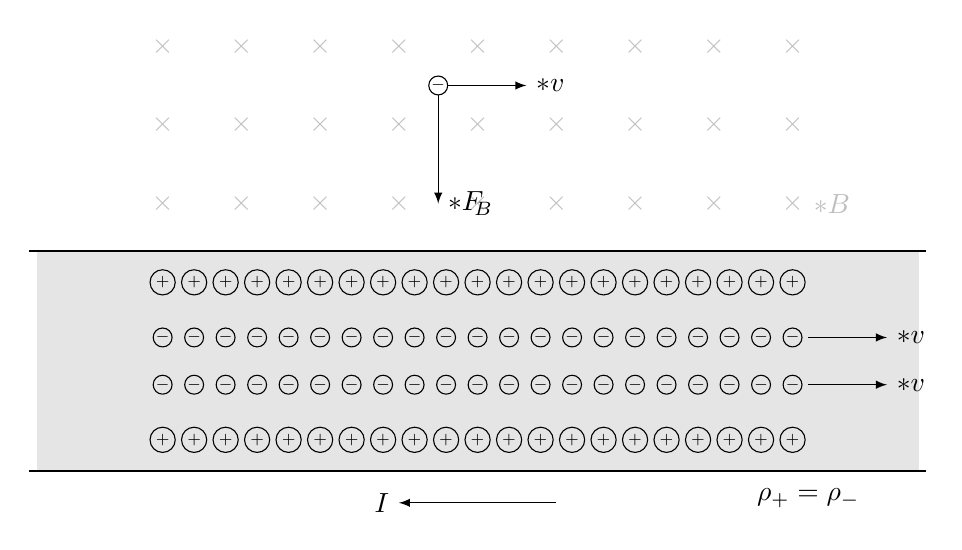
\begin{tikzpicture}[scale=2]
    \draw[thick](-2.85,+0.7)--(+2.85,+0.7);
    \draw[thick](-2.85,-0.7)--(+2.85,-0.7);
    \fill[black,fill opacity=0.1] (-2.8,0.7) rectangle (2.8,-0.7);
    \foreach \i in {-2,-1.8,...,2}
    {
        \draw (\i,+0.5) circle (0.08);
        \node at(\i,+0.5) {\tiny $+$};
        \draw (\i,-0.5) circle (0.08);
        \node at(\i,-0.5) {\tiny $+$};
    }
    \foreach \i in {-2,-1.8,...,2}
    {
        \draw (\i,+0.15) circle (0.06);
        \node at(\i,+0.15) {\tiny $-$};
        \draw (\i,-0.15) circle (0.06);
        \node at(\i,-0.15) {\tiny $-$};
    }
    \draw[-latex](2.1,+0.15)--(2.6,+0.15);
    \draw[-latex](2.1,-0.15)--(2.6,-0.15);
    \node[right] at (2.6,+0.15){$\vb*{v}$};
    \node[right] at (2.6,-0.15){$\vb*{v}$};

    \foreach \i in {-2,-1.5,...,2}
    {
        \foreach \j in {1,1.5,2}
        \node[black!25!white] at (\i,\j) {$\times$};
    }

    \draw (-0.25,1.75) circle (0.06);
    \node at(-0.25,1.75) {\tiny $-$};
    \draw[-latex](-0.19,1.75)--(0.31,1.75);
    \node[right] at (0.31,1.75){$\vb*{v}$};
    \draw[-latex](-0.25,1.69)--(-0.25,1.00);
    \node[right] at (-0.25,1.00){$\vb*{F}_{\hspace{-2pt}B}$};
    \node[black!25!white] at (2.25,1.0) {$\vb*{B}$};

    \draw[-latex] (0.5,-0.9)--(-0.5,-0.9) node[left] {$I$};
    \node[below] at (2.1,-0.75) {$\rho_{+}=\rho_{-}$};

    \clip(-2.85,-1) rectangle (2.85,2.1);
\end{tikzpicture}
